\section{Abelian Anyons II}

Consider a gapped $d$-dimensional Hamiltonian $H$ with short-ranged interaction. Supports $H$ supports a particle-like excitation. Last class, we looked at the single and multi-particle Berry phase for closed paths of such particle-like excitations. We argued that the most general form for the $n$-particle Berry phase took the form:
\begin{equation}\label{eq:berryphasedecomp}
    \theta_B(\Gamma) = \theta_{s-r}(\Gamma) + \theta_{\text{top}}(\Gamma)
\end{equation}
where the short-ranged piece looks like:
\begin{equation}
    \theta_{s-r}(\Gamma) = \sum_{i=1}^n \int_{\Gamma}\left(\gv{\mathcal{A}}(\v{r}_i) + \sum_j \gv{\mathcal{B}}(\v{r}_i, \v{r}_j) + \sum_{jk}\gv{\mathcal{C}}(\v{r}_i, \v{r}_j, \v{r}_k)\right)d\v{r}_i
\end{equation}
where the multi-particle terms are short-ranged. The topological term we discussed only depends on the topological class of $\Gamma$ (c.f. the short-range part is non-universal and depends on the microscopic details of the path). This topological term will be what informs the exchange statistics. We now ask - what are the possible $\theta_{\text{top}}$ terms that can appear in Eq. \eqref{eq:berryphasedecomp}? An important constraint is that it must be multiplicative under composition:
\begin{equation}\label{eq:comp}
    e^{i\theta_{\text{top}}(\Gamma_2 \circ \Gamma_1)} = e^{i\theta_{\text{top}}(\Gamma_2)}e^{i\theta_{\text{top}}(\Gamma_1)}.
\end{equation}
This is because $e^{i\theta_B}$ and $e^{i\theta_{s-r}}$ both obey this property. Thus, we look for topological terms that obey this property. Formally, this amounts to finding 1-D representations of the braid group.

\begin{center}
    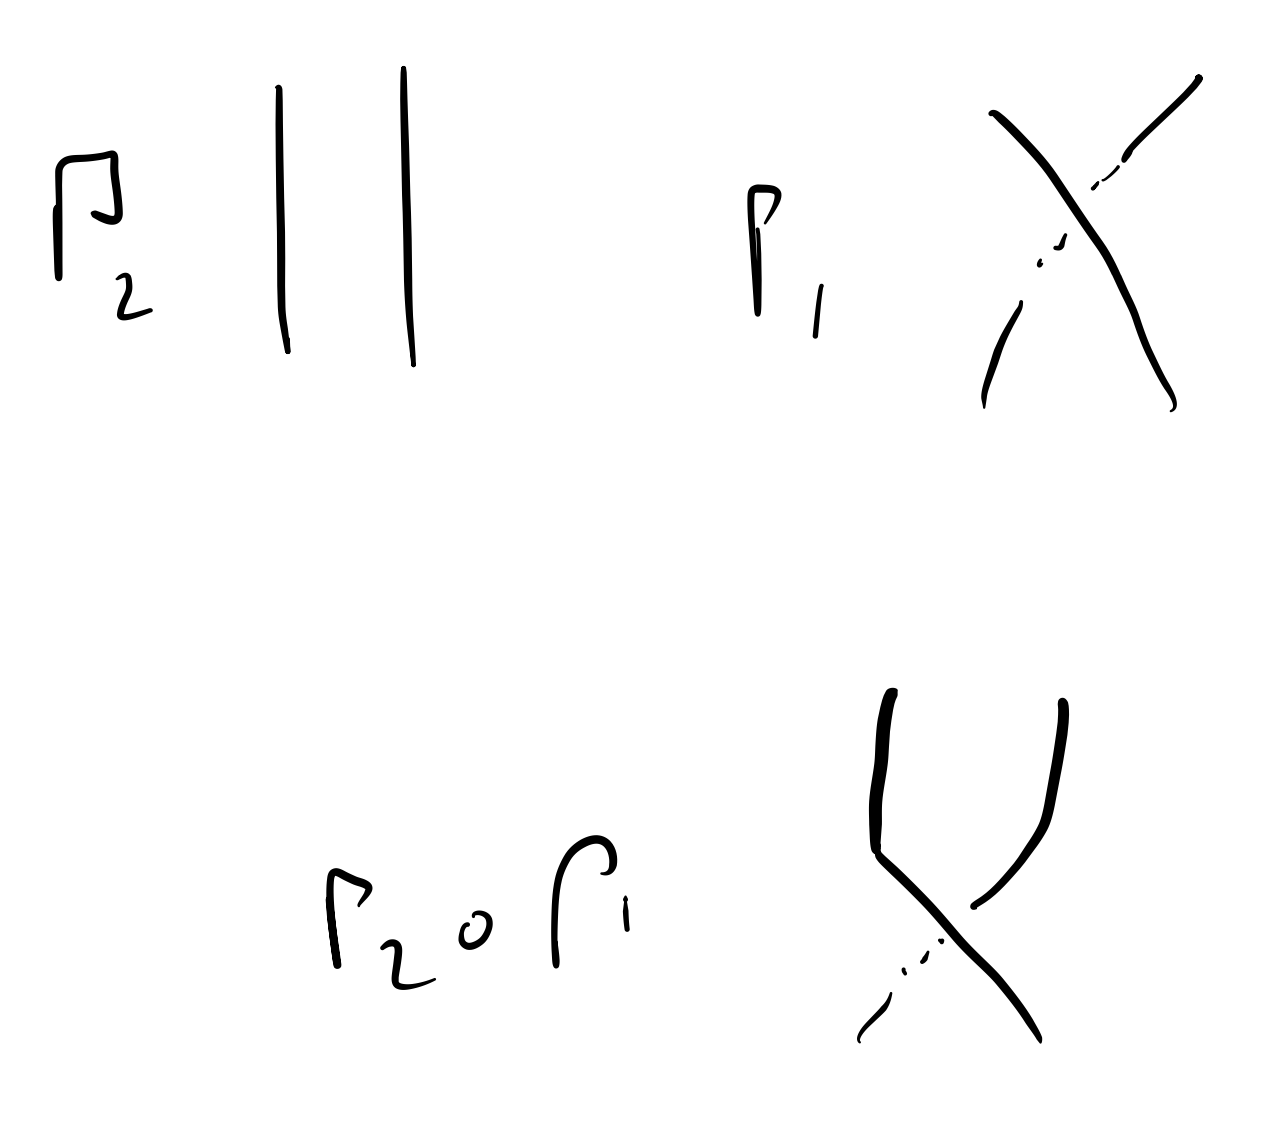
\includegraphics[scale=0.3]{Lectures/Images/lec5-pathcomp.png}
\end{center}

\subsection{Topological Berry Phase in 3D}
For simplicity, we focus on 2-particle paths. There are 2 such paths in 3D; one where the particles do not exchange, and then one without (picture below slightly misleading because it's hard to draw in 3+1D). We might ask; what if we do 2 exchanges? In 2D we cannot unwrap this, but in 3D a double exchange can be continuously deformed to no exchanges (by using the third spatial dimension).

\begin{center}
    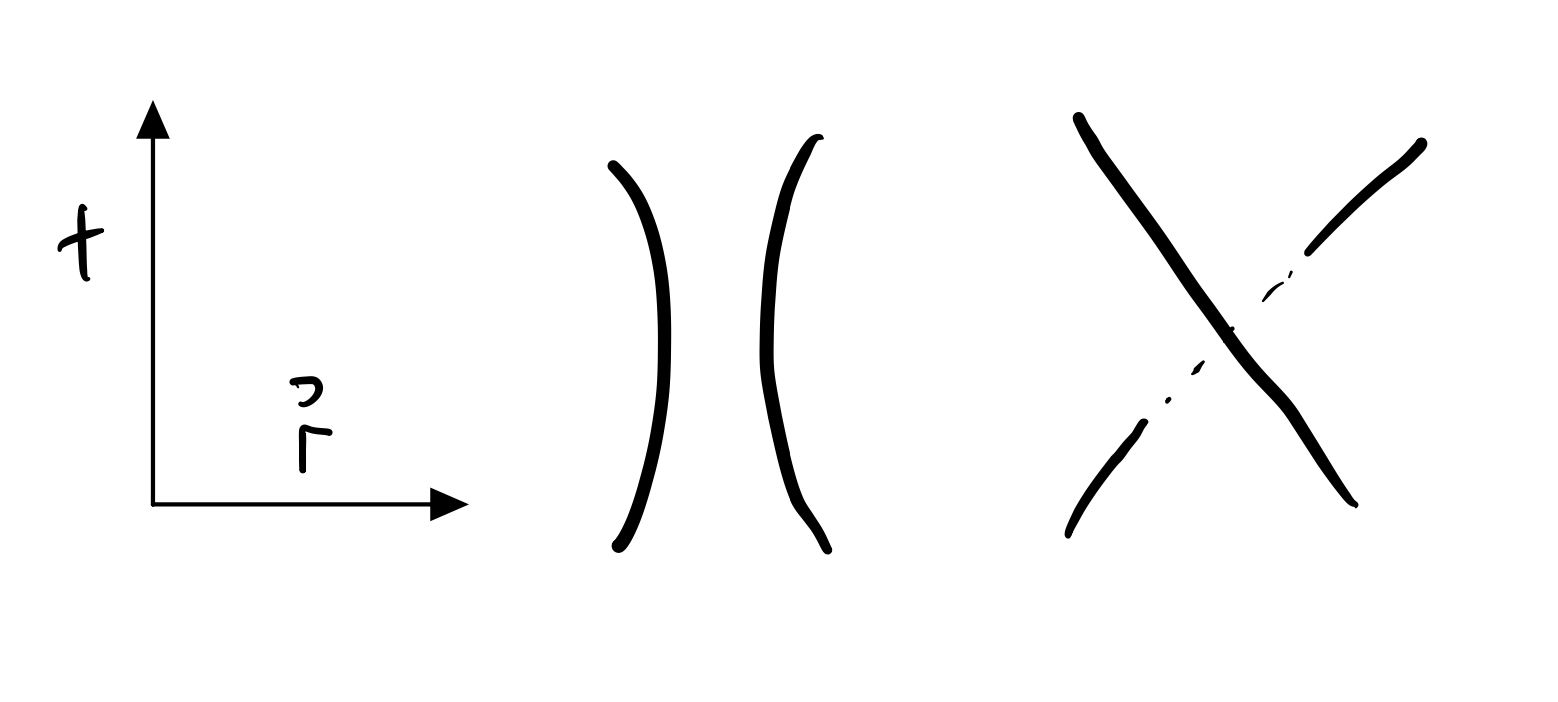
\includegraphics[scale=0.35]{Lectures/Images/lec5-3dbraids.png}
\end{center}

There are then two possible values for the topological Berry phase:
\begin{equation}
    e^{i\theta_{\text{top}}(\text{no exchange})} = a, \quad  e^{i\theta_{\text{top}}(\text{exchange})} = b
\end{equation}
By Eq. \eqref{eq:comp}:
\begin{equation}
    e^{i\theta_{\text{top}}(\text{double exchange})} = b^2
\end{equation}
but also, since a double exchange can be topologically deformed to the trivial path:
\begin{equation}
    e^{i\theta_{\text{top}}(\text{double exchange})} = e^{i\theta_{\text{top}}(\text{no exchange})} = a
\end{equation}
So then we obtain the constraint:
\begin{equation}
    b^2 = a
\end{equation}
We can write a very similar equation if we do a trivial path twice; again by Eq. \eqref{eq:comp}
\begin{equation}
    e^{i\theta_{\text{top}}(\text{double no exchange})} = a^2
\end{equation}
but this is also topologically equivalent to the trivial path/a single no exchange path:
\begin{equation}
    e^{i\theta_{\text{top}}(\text{double no exchange})} = e^{i\theta_{\text{top}}(\text{no exchange})} = a
\end{equation}
and thus:
\begin{equation}
    a^2 = a
\end{equation}
So, we have two solutions:
\begin{enumerate}
    \item $a = 1$, $b = 1$ - this is the case where there is no Berry phase for an exchange. This is the physical definition of a boson.
    \item $a = 1$, $b = -1$ - this is the case where an exchange gives a Berry phase of -1. This is the physical definition of a fermion.
\end{enumerate}
The modern view is that fermions have nonlocal behaviour, and the anticommutation relations are a way to package this nonlocality in a local way.

\subsection{Topological Berry Phase in 2D}
Again, we focus on 2-particle paths (this fully determines the $n$-particle behaviour). Unlike in 3D, we get many topological classes, with different classes corresponding to different braids.

\begin{center}
    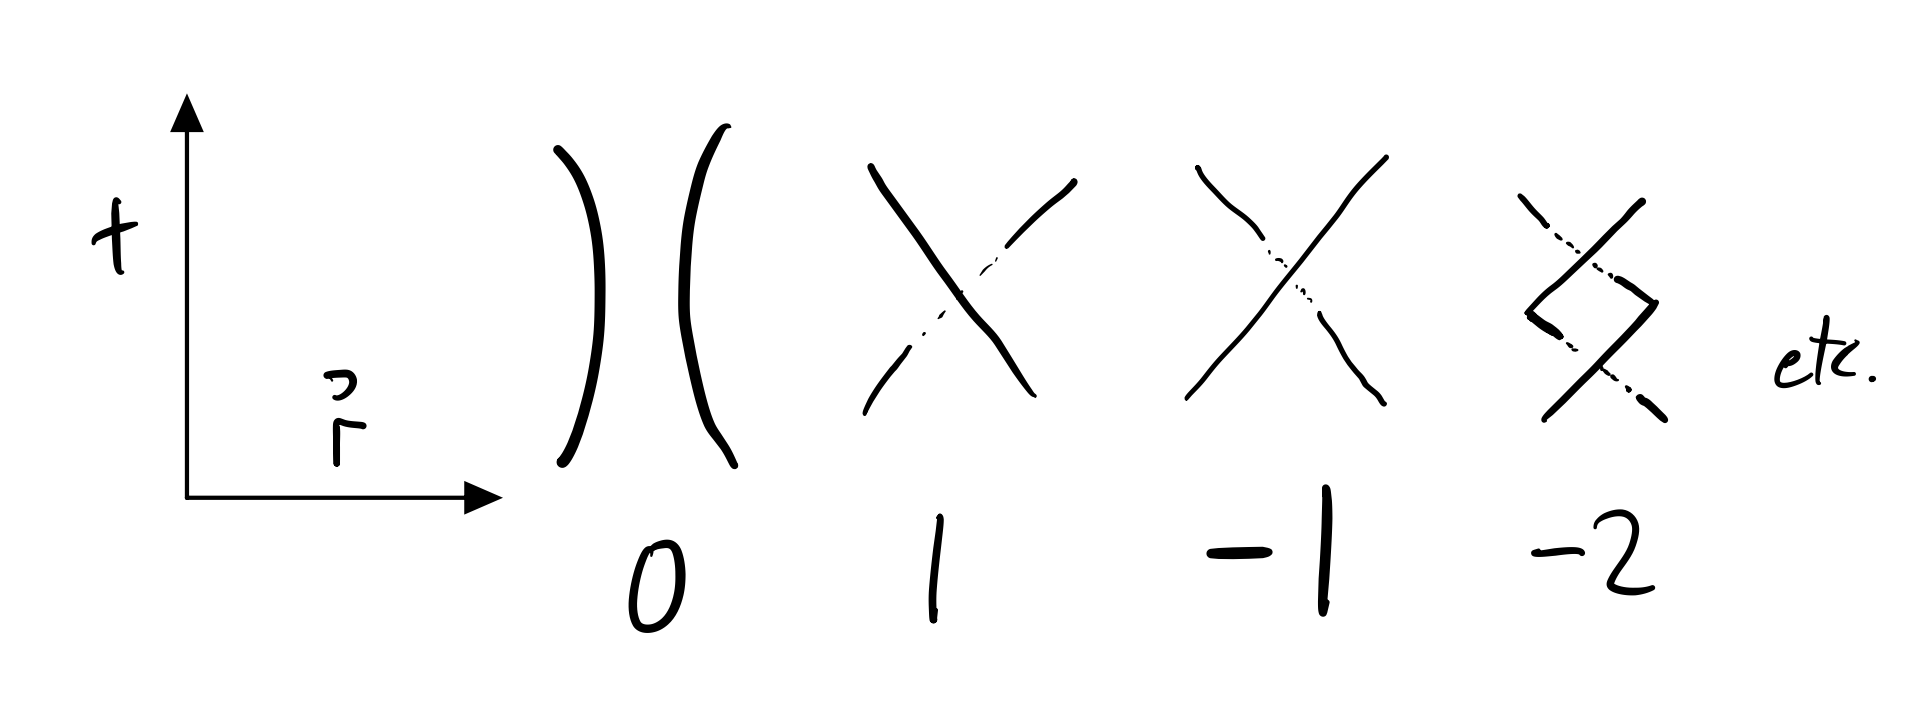
\includegraphics[scale=0.35]{Lectures/Images/lec5-2dbraids.png}
\end{center}

We can label braids by the number of times particles exchange in the clockwise direction. We let:
\begin{equation}
    e^{i\theta_{\text{top}}(\text{n clockwise exchanges})} = a_n
\end{equation}
Then, we know by Eq. \eqref{eq:comp} that:
\begin{equation}
    a_n = a_1^n
\end{equation}
Since we have no other constraints, we can let:
\begin{equation}
    a_1 = e^{i\theta}
\end{equation}
Then:
\begin{equation}
    e^{i\theta_{\text{top}}(\text{n clockwise exchanges})} = e^{in\theta}
\end{equation}
The $\theta$ is thus known as the ``statistical angle of excitations''. There are three cases:
\begin{enumerate}
    \item $\theta = 0$ - no phase from exchanges - bosons
    \item $\theta = \pi$ - $-1$ phase from exchanges - fermions
    \item $\theta \neq 0, \pi$ - some other $e^{i\theta}$ phase from excitations - anyons
\end{enumerate}

\subsection{Generalization to multiple anyon types}
Suppose $H$ supports several types of particle excitations $A = \set{a, b, \ldots}$. We can then consider multi-particle closed paths $\Gamma$, for example:

\begin{center}
    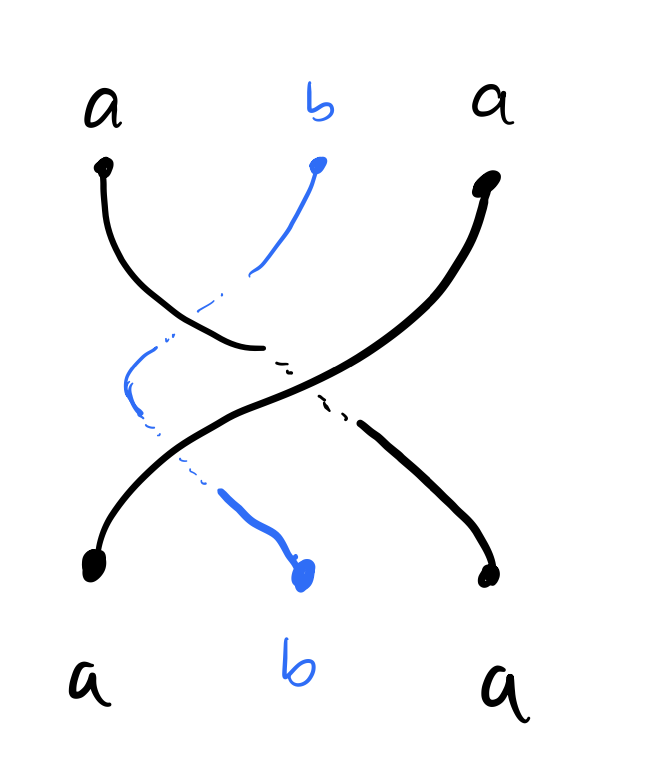
\includegraphics[scale=0.35]{Lectures/Images/lec5-2dbraidexample.png}
\end{center}

In this case, what are the possible topological terms? Without going through the entire argument, $\theta_{\text{top}}(\Gamma)$ is characterized by multiple statistical angles (we consider the 2-particle case, which again characterizes all multi-particle paths):
\begin{enumerate}
    \item $\set{e^{i\theta_a}: a \in A}$; ``exchange statistics of $a$''
    \begin{center}
        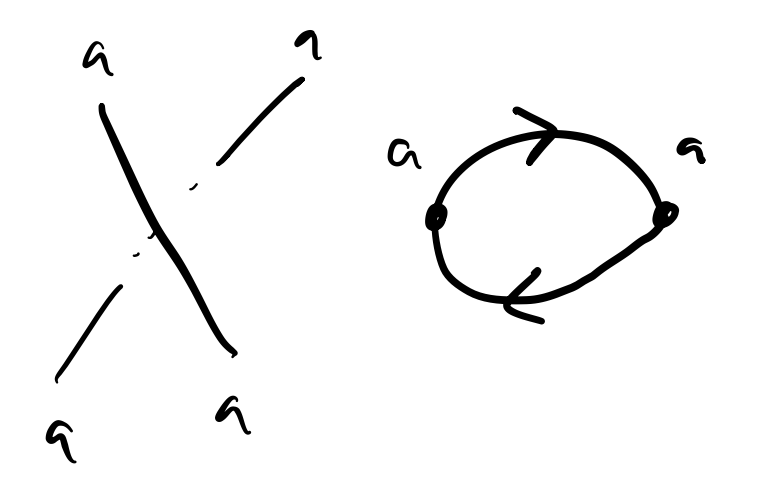
\includegraphics[scale=0.35]{Lectures/Images/lec5-exchange.png}
    \end{center}
    \item $\set{e^{i\theta_{ab}}: a, b \in A}$ ``mutual statistics'' 
    \begin{center}
        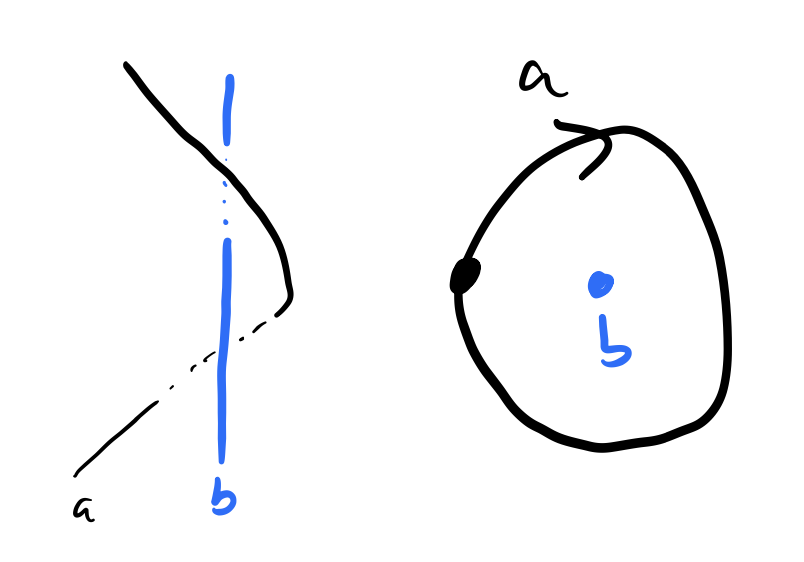
\includegraphics[scale=0.35]{Lectures/Images/lec5-mutual.png}
    \end{center}
\end{enumerate}
There are some important constraints on the statistical angles:
\begin{enumerate}
    \item $e^{i\theta_{ab}} = e^{i\theta_{ba}}$ - this is because wrapping $a$ around $b$ is topologically equivalent to wrapping $b$ around $a$.
    \begin{center}
        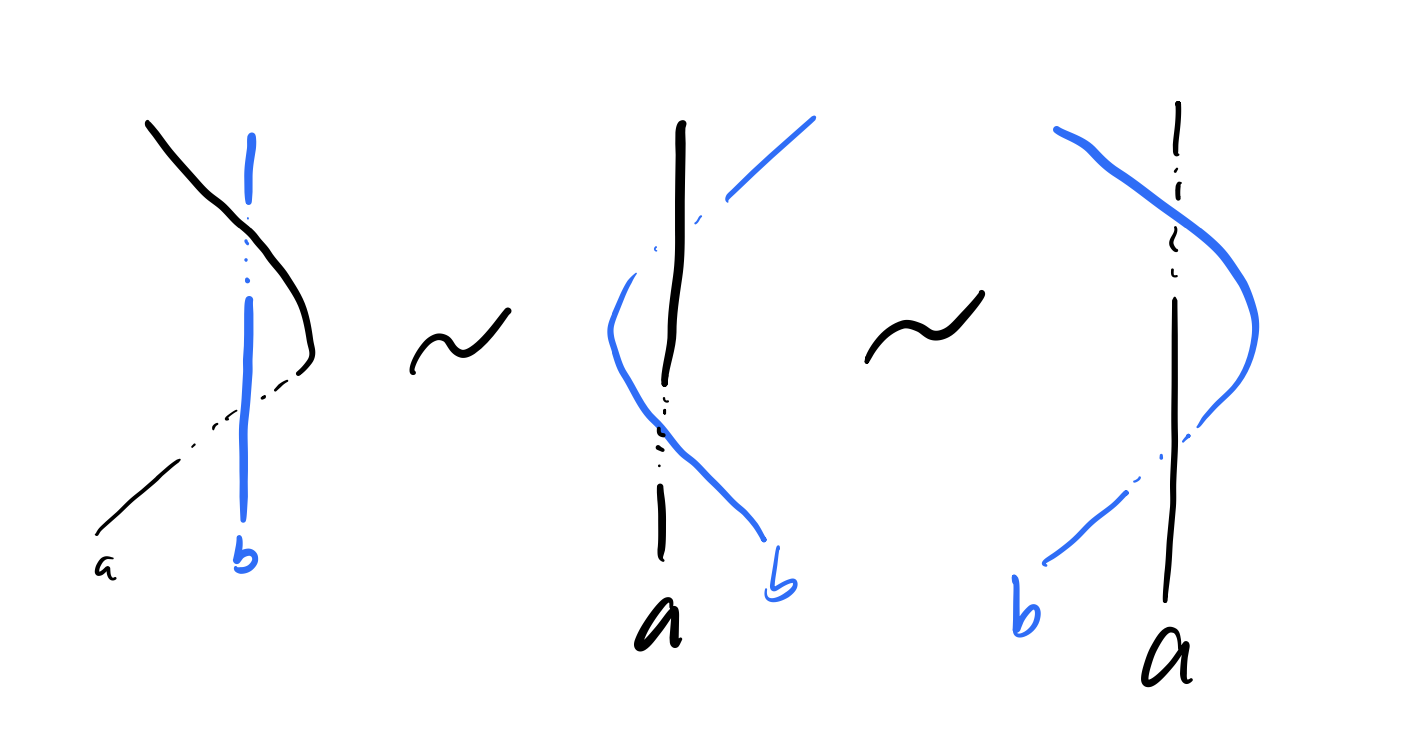
\includegraphics[scale=0.35]{Lectures/Images/lec5-mutualrelation.png}
    \end{center}
    \item $e^{i\theta_{aa}} = e^{2i\theta_a}$ - wrapping $a$ around an $a$ is topologically equivalent to a double exchange.
    \begin{center}
        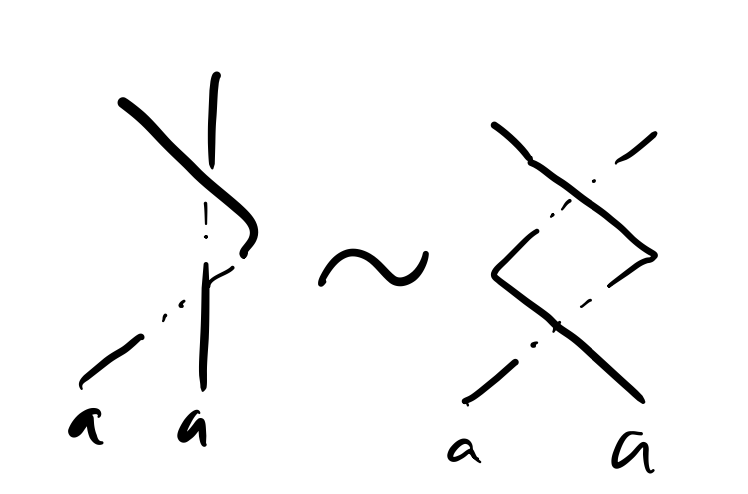
\includegraphics[scale=0.35]{Lectures/Images/lec5-exchangerelation.png}
    \end{center}
\end{enumerate}
Terminology: A ``non-trivial'' anyon $a$ is a particle such that $e^{i\theta_{ab}} \neq 1$ for some $b$ (allowing for $b = a$). In other words, an anyon is a particle which braids non-trivially with another particle. Note that this means that some particles may have trivial exchange statistics, but still be anyons by virtue of non-trivial mutual statistics. This will be the case for the Toric code, where $e, m$ individually have trivial exchange statistics but braid non-trivially.

So, let us summarize. For a general gapped system with particle-like excitation, the topological Berry phase is completely characterized by the exchange statistics and the mutual statistics. Now, to have a concrete example, let's compute these both for the toric code.

\subsection{Anyons in the Toric Code}
Let's compute the mutual statistics of the charge and flux excitations. We denote the mutual statistics by $e^{i\theta_{em}}$ (we denote the charge by $e$ and the flux by $m$, as in Gauge theory). To compute this, we have to somehow extract the topological part of the Berry phase. To this end, we compare 2 different paths such that the uninteresting/short ranged parts of the Berry phase cancel out.
\begin{center}
    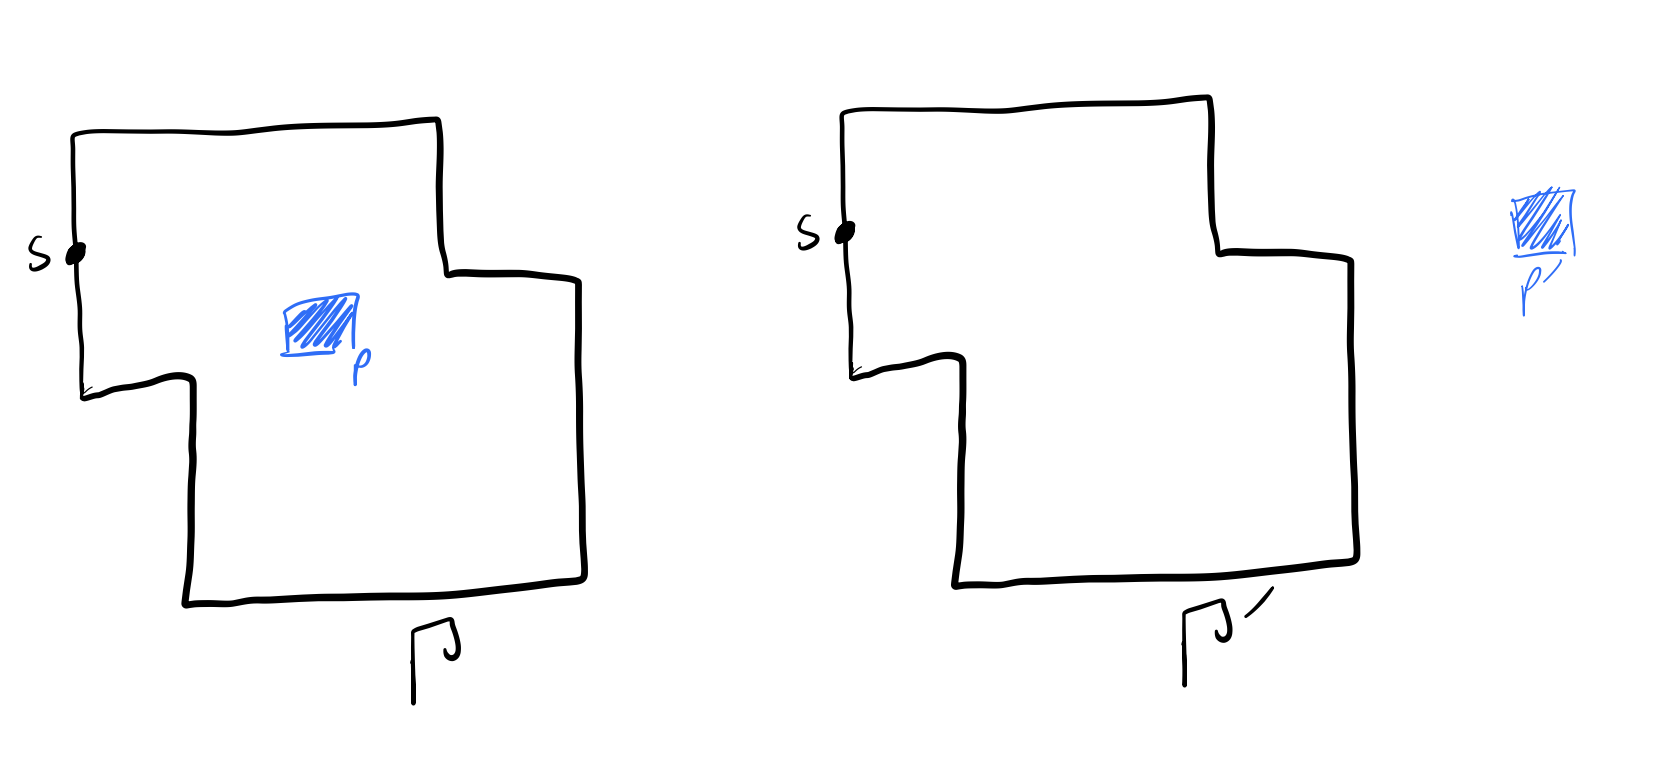
\includegraphics[scale=0.35]{Lectures/Images/lec5-toricpaths.png}
\end{center}

We can write this as:
\begin{equation}
    \theta_B(\Gamma) - \theta_B(\Gamma') = [\theta_{s-r}(\Gamma) - \theta_{s-r}(\Gamma')] + [\theta_{\text{top}}(\Gamma) - \theta_{\text{top}}(\Gamma')]
\end{equation}
By construction, the $s-r$ parts cancel because locally the two paths look exactly the same (locally, you don't see the flux you are surrounding or avoiding). Further, we notice that $\Gamma'$ is topologically trivial because $\Gamma'$ can be shrunk to a point (there is no plaquette inside it). Thus:
\begin{equation}
    \theta_B(\Gamma) - \theta_B(\Gamma') = \theta_{\text{top}}(\Gamma) = \theta_{\text{em}}
\end{equation}
Likewise, if $\Gamma, \Gamma'$ are adiabatic cycles, then:
\begin{equation}
    \theta(\Gamma) - \theta(\Gamma') = [\theta_B(\Gamma) - \theta_B(\Gamma')] + [\theta_{\text{dyn}}(\Gamma) - \theta_{\text{dyn}}(\Gamma')] = \theta_{\text{em}}
\end{equation}
as the dynamical phase between the two cycles cancel, as well. In fact, $\Gamma, \Gamma'$ do not have to be adiabatic; they can be composed out of any sequence of \emph{local} ``movement operators'', and we will still get:
\begin{equation}
    \theta(\Gamma) - \theta(\Gamma') = \theta_{\text{em}}
\end{equation}
and this will be how we compute $\theta_{\text{em}}$ for the toric code. Let's try this. Notice that $Z_j$ moves a charge:
\begin{center}
    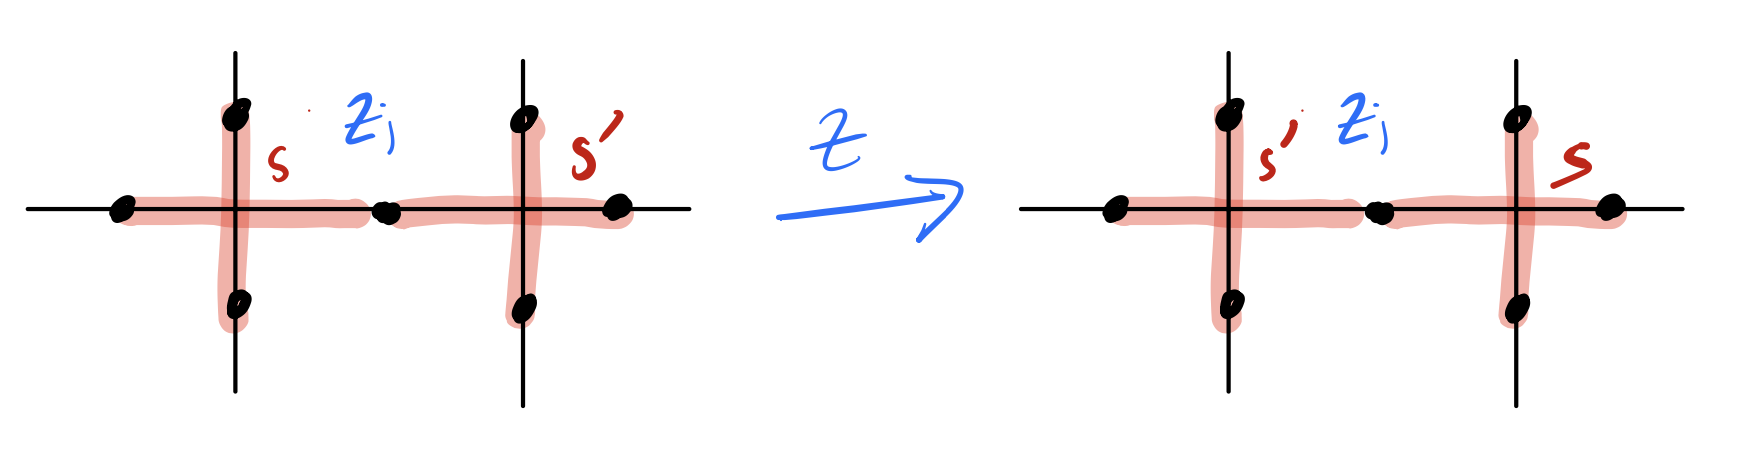
\includegraphics[scale=0.35]{Lectures/Images/lec5-movecharges.png}
\end{center}

and this is because $Z_j$ anticommutes with $A_s, A_{s'}$, resulting in:
\begin{equation}\label{eq:applyZ}
    \begin{split}
        Z_j\ket{a_s = 1, a_{s'} = 1} &= \ket{a_s = -1, a_{s'} = -1}
        \\ Z_j\ket{a_s = -1, a_{s'} = -1} &= \ket{a_s = 1, a_{s'} = 1}
        \\ Z_j\ket{a_s = 1, a_{s'} = -1} &= \ket{a_s = -1, a_{s'} = 1}
        \\ Z_j\ket{a_s = -1, a_{s'} = 1} &= \ket{a_s = 1, a_{s'} = -1}
    \end{split}
\end{equation}